\chapter{Introduction}

\section{Research Motivation}

Since its inception, the Internet has served a vast user base that wishes to communicate with one another and spread information. By design, the Internet is a platform that should provide unfiltered content to users. In many cases this content may otherwise be inaccessible by traditional media outlets such as radio or TV. Originally designed to aid government researchers share information, its open and transparent foundation has since changed. Across the globe, governments and other entities are censoring the internet by network manipulation, legislative pressure or otherwise. This is a global threat to fundamental internet user rights and should be treated as such. It is for these reasons that this area ought to be investigated more thoroughly.

Although censorship of certain content (CSAM, pirated entertainment) is widely considered appropriate, normalising this has far reaching consequences on user privacy and free speech. The importance of establishing a quantitative approach to measuring internet censorship cannot be overstated as users are unaware of invisible content in most cases. As a result, the state has a large influence over what ideas can propagate within its borders. Various open-source and community-led projects aimed at addressing this issue. Notable examples include the Tor project, OONI, Tails OS and others. However, it is coming to light that this technology is becoming deprecated. In 2022, German police were able to make an arrest after de-anonymising Tor traffic using timing analysis \cite{TorDeanonymization}. This highlights the large dichotomy between what users believe governments are capable of and reality. 

\subsection{User Rights \& Privacy}
In discussing internet user rights and how censorship occurs, it is important to mention anonymity and user privacy. DRI, a non-profit that challenges the Irish government on data retention issues is an independent, non-profit organization. They state on their website, that users have "a right to digital privacy [\&] data security." \cite{digital_rights_ireland} Individuals' freedom to access information and be anonymous are inherently linked, however very separate issues. Though censors may actively engage in deanonymisation efforts, potentially using methods described below, this research is focused on internet censorship.


For the above reasons, the increasingly pervasive censorship done by governments and corporations around the world is concerning. The sheer number of individuals affected by internet censorship and the lack of transparency are strong motives for more extensive research.

\section{Background}
\subsection{Global Internet Censorship}
Experts suggest that censorship on the internet is increasing at an alarming rate. “The majority of countries that censor content do so across all four themes, although the depth of the filtering varies. The study confirms that 40 percent of these 2,046 websites can only be reached by an 
encrypted connection (denoted by the "HTTPS" prefix on a web page, a voluntary upgrade from "HTTP").” \cite{Zittrain2017Censorship} It is also clear that more and more countries are viewing this as a necessary solution to the unique problems they have. Whether this is appropriate or not, it is happening, and users should be aware of this. 

Governments have a vested interest in maintaining control over telecommunications industries and public internet use. Whether protecting state secrets, preventing cyber crime piracy or acts of terrorism, insulating from perceived negative influence, aiding in the creation of propaganda or otherwise; a large majority of governments choose to exercise inordinate control over the 
information available to its public.  

As more governments and entities began to engage in this, it became increasingly important to hold them accountable. As a result, the ‘Enemies of the Internet’ list was devised. It contains the governments and entities that actively engage in the repression of online freedoms, in the form of censorship and surveillance. As of 2014, there were 19 governments that fit this criterion but by now this number has likely increased. \cite{RSFEnemiesInternet2014} Traditionally, censorship involved monitoring a handful of media and cutting undesirable content, potentially replacing this with a message more in line with the agenda and norms of the locale. However, with the advent of the internet, this distribution of information became decentralised and thus allowed for more expression and freedom in the content consumed by a user. As a result, censorship has become more difficult to conduct, but potentially easier to get away with. Nowadays, governments leverage points of control, network-level filtering and many other techniques to block undesirable content.


\section{Project Scope}
Below is an outline of the goals for the thesis. The stretch goal is to contribute to the OONI project. A more attainable contribution is to merge resources in order to compile a better sensitive domain list that is specific to Ireland and Israel. This would improve the testing capability for the locations being considered.

\begin{figure}
    \centering
    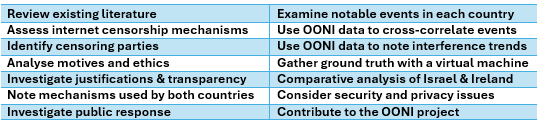
\includegraphics[width=1\linewidth]{introduction/thesisgoals.png}
    \caption{Goals of the research}
    \label{fig:enter-label}
\end{figure}
